To check the light-tightness of the dark box, the PMT dark current was measured before and after covering the setup by a special black blanket from Thorlabs \cite{BlackBlancket}, that prevents external photons from entering the system. No statistically significant differences was observed between the covered and uncovered setup, which indicates that the black box is sufficiently light tight. The optimal PMT HV was obtained by finding the voltage plateau at which the electron collection efficiency in the first dynode was practically $100\%$. In absence of fibers, the PMT output current was measured for different PMT supply voltages, between $0$ and $500~\volt$, first with the LED off (PMT dark current) and then with the LED current at $1~\milli\ampere$. The number of photons detected by the PMT (difference between both spectra) is plotted in Figure \ref{fig:PlateauNoGainPMT}. As it can be seen, the plateau starts at voltages higher than $150~\volt$. The selected voltage for the characterization was $250~\volt$.

\begin{figure}[h]
\centering
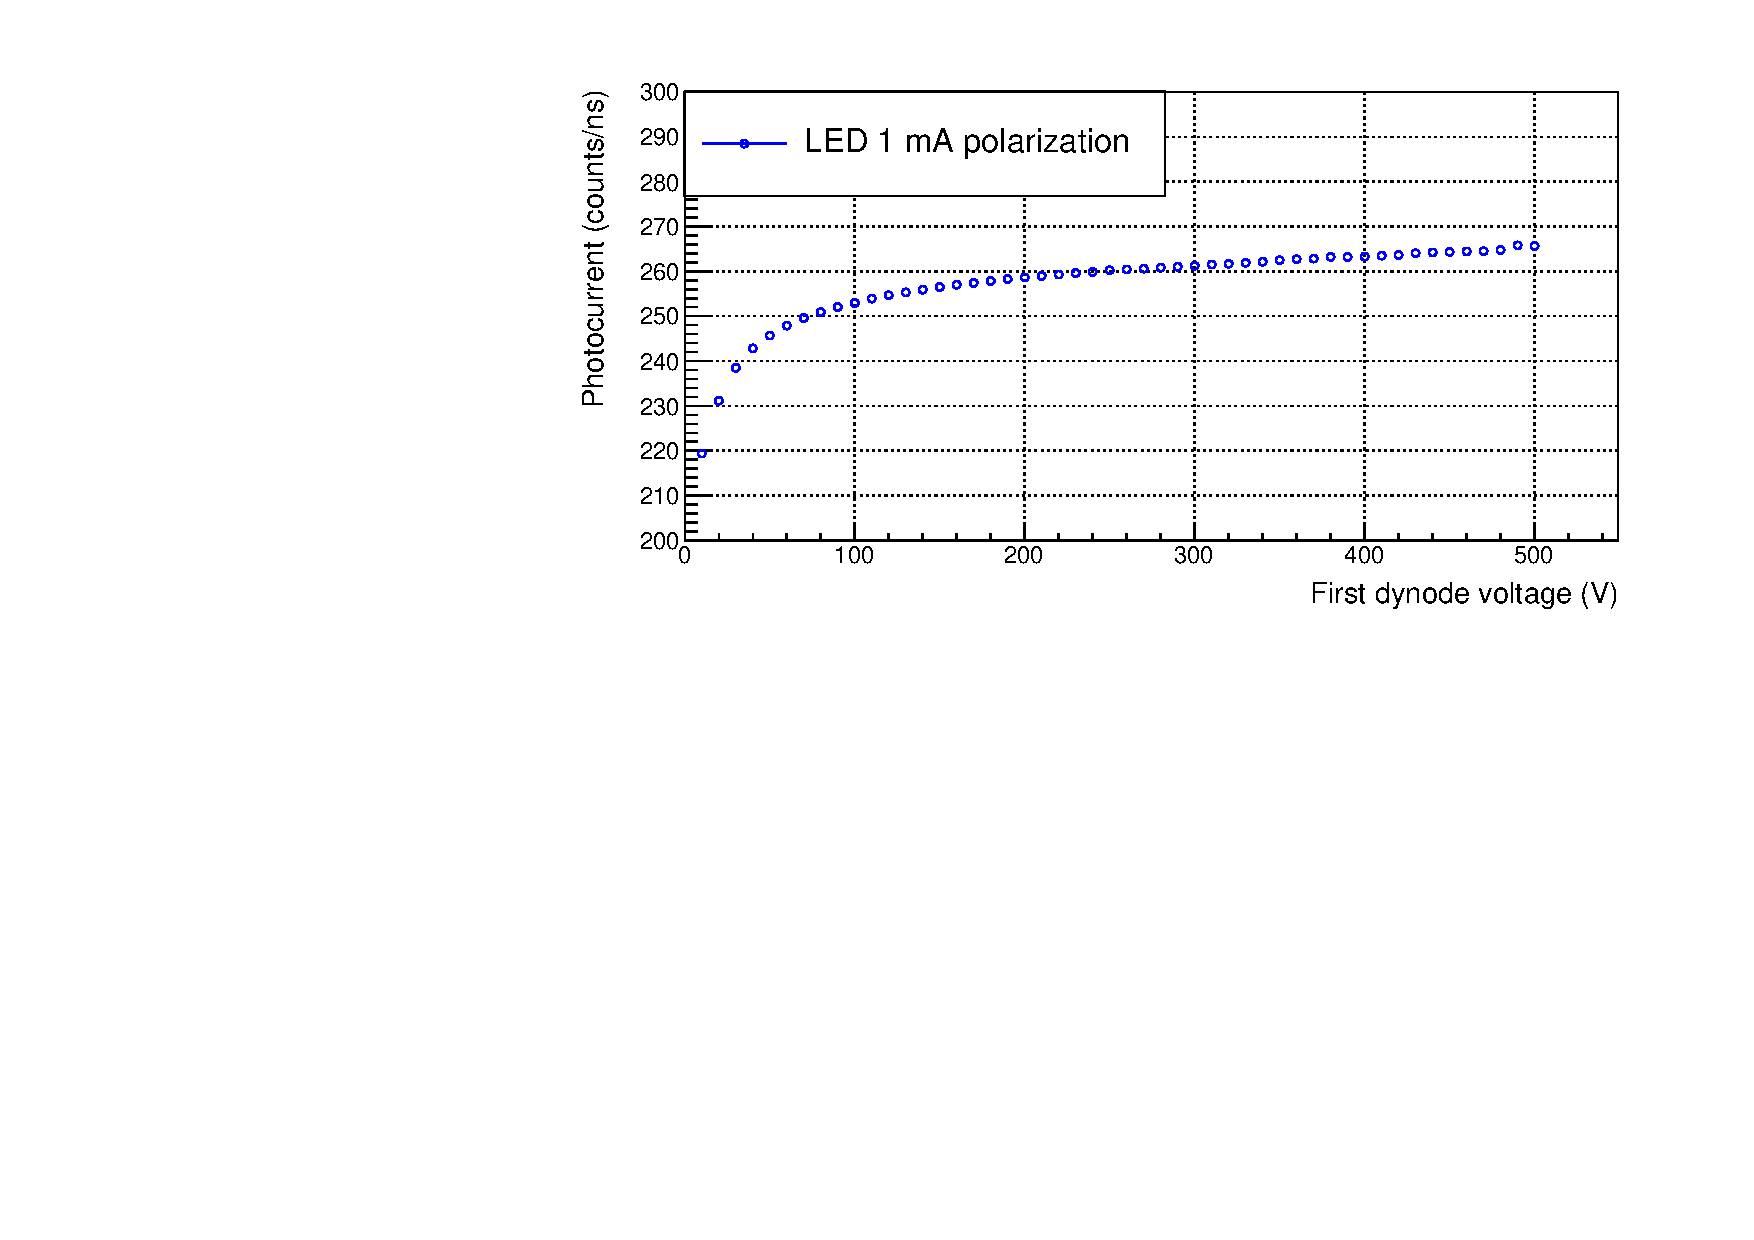
\includegraphics[scale=0.7]{4ResearchAndDevelopments/41Fibers/PCBNoGainPlateau_Calibrated.pdf}
\caption{PMT photocurrent as a function of the first dynode voltage. Error bars are smaller than dot size.\label{fig:PlateauNoGainPMT}}
\end{figure}

The linear response of the PMT was verified. The LED was powered in current mode with intensities ranging from 0 to $10~\milli\ampere$, that cover numbers of photons from tritium events (tens of $~\text{photons}/\nano\second$) to high activities ($\sim 2500~\text{photons}/\nano\second$). The linearity test of the PMT was performed without fibers. Several collimators were used to reduce the number of photons that reach the PMT. The results in the low and high illumination cases are plotted in Figure \ref{fig:LinearityRangesOfPMT}, in which no saturation of the PMT response is observed.

\begin{figure}
\centering
    \begin{subfigure}[b]{1\textwidth}
    \centering
    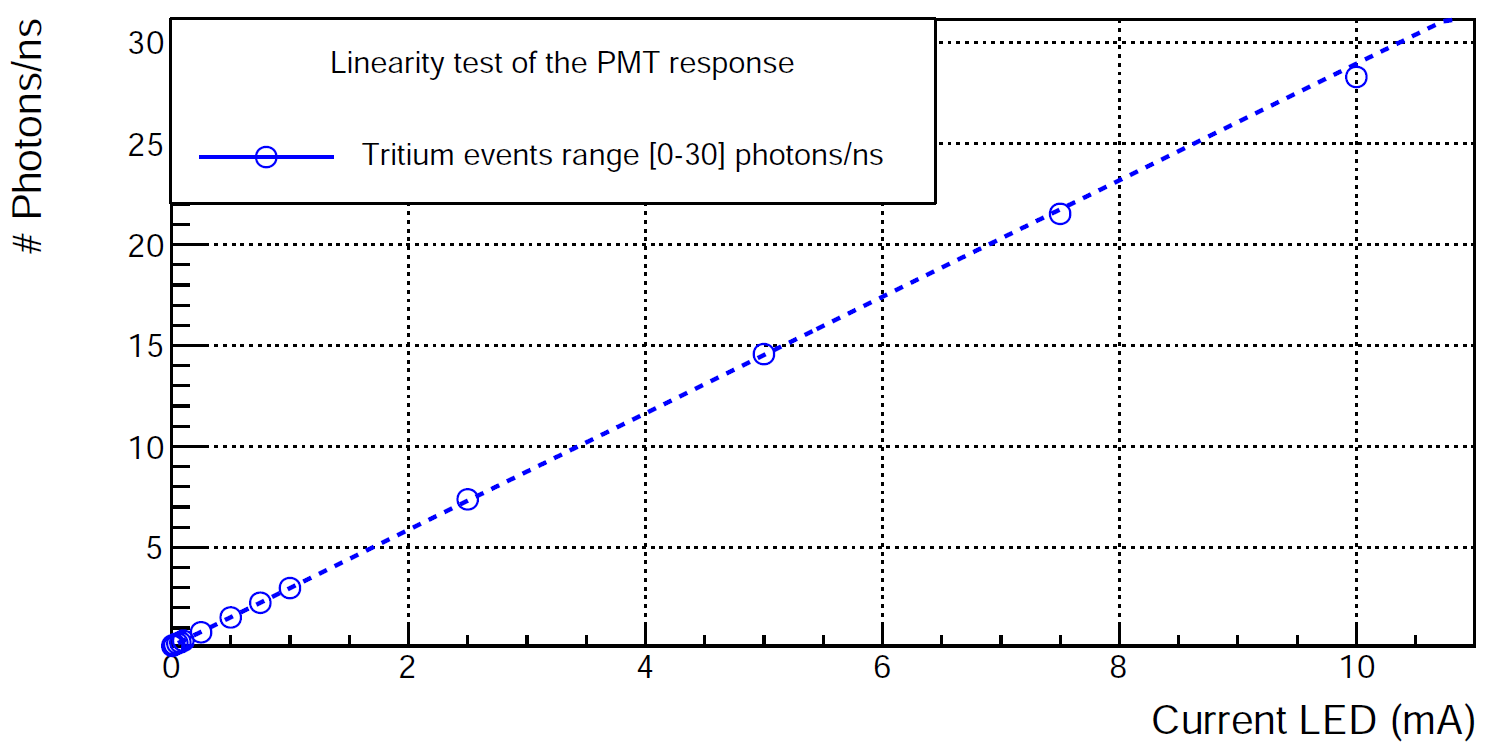
\includegraphics[scale=0.4,width=\textwidth]{4ResearchAndDevelopments/41Fibers/Linearity_test_0_30_range.png}  
    \caption{\label{subfig:LinearityTritiumRange}}
    \end{subfigure}
    \hfill
    \begin{subfigure}[b]{1\textwidth}
    \centering
    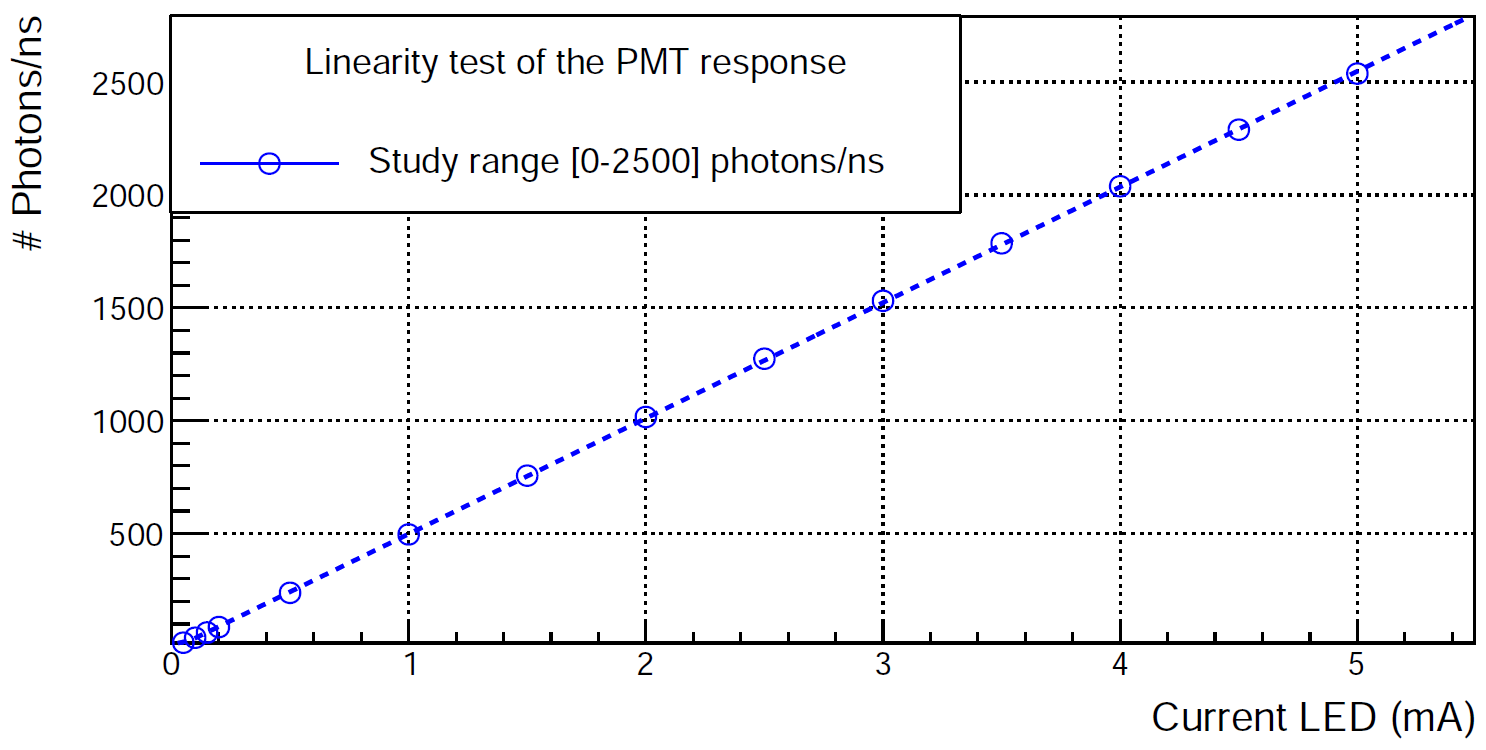
\includegraphics[scale=0.4, width=\textwidth]{4ResearchAndDevelopments/41Fibers/Linearity_test_0_2500_range.png}  
    \caption{\label{subfig:LinearityStudyRange}}
    \end{subfigure}
 \caption{Rate of photons measured by the PMT as a function of the LED current. a) Response of the PMT in the intensity range of tritium events. b) Response of the PMT in the range $0-2500~\text{photons}/\nano\second$. Error bars are smaller than the dot size.}
 \label{fig:LinearityRangesOfPMT}
\end{figure}